\documentclass[tikz,border=10pt]{standalone}
% Shared preamble for the CenterTask panel files (panel_a/b/c.tex).
% Edit colours and node styles here, once.
\usepackage{amsmath}
\usetikzlibrary{arrows.meta,positioning,calc}

% category colours as in ColorCategoryMap.m: 1=Short/Orange, 2=Mid/Green, 3=Long/Blue
\definecolor{catShort}{RGB}{243,178,132}
\definecolor{catMid}{RGB}{158,209,172}
\definecolor{catLong}{RGB}{157,188,234}

\tikzset{ctpanel/.style={
  font=\sffamily,
  band/.style={rounded corners=6pt, fill=black!7, draw=none, inner sep=8pt, minimum height=1.15cm},
  unit/.style={circle, fill=catMid!60, draw=none, minimum size=0.95cm, inner sep=0pt},
  flow/.style={-{Latex[length=2.2mm]}, line width=0.8pt},
  rowlab/.style={anchor=east, font=\sffamily\large},
  now/.style={fill=catShort!55, rounded corners=3pt, inner sep=3pt},
  stage/.style={rounded corners=6pt, fill=black!8, draw=none, inner sep=8pt, minimum height=1.2cm, align=center},
  target/.style={circle, minimum size=0.9cm, inner sep=0pt, draw=none, font=\sffamily\scriptsize, text=black!75},
  axis/.style={line width=0.6pt},
}}


% ---------------------------------------------------------------------
%  Coupling pipeline: how network 1's trial-level read-out becomes a
%  constant input to network 2, and how network 2's simulated trajectory
%  is checked back against network 1's timing heads.
% ---------------------------------------------------------------------

\begin{document}
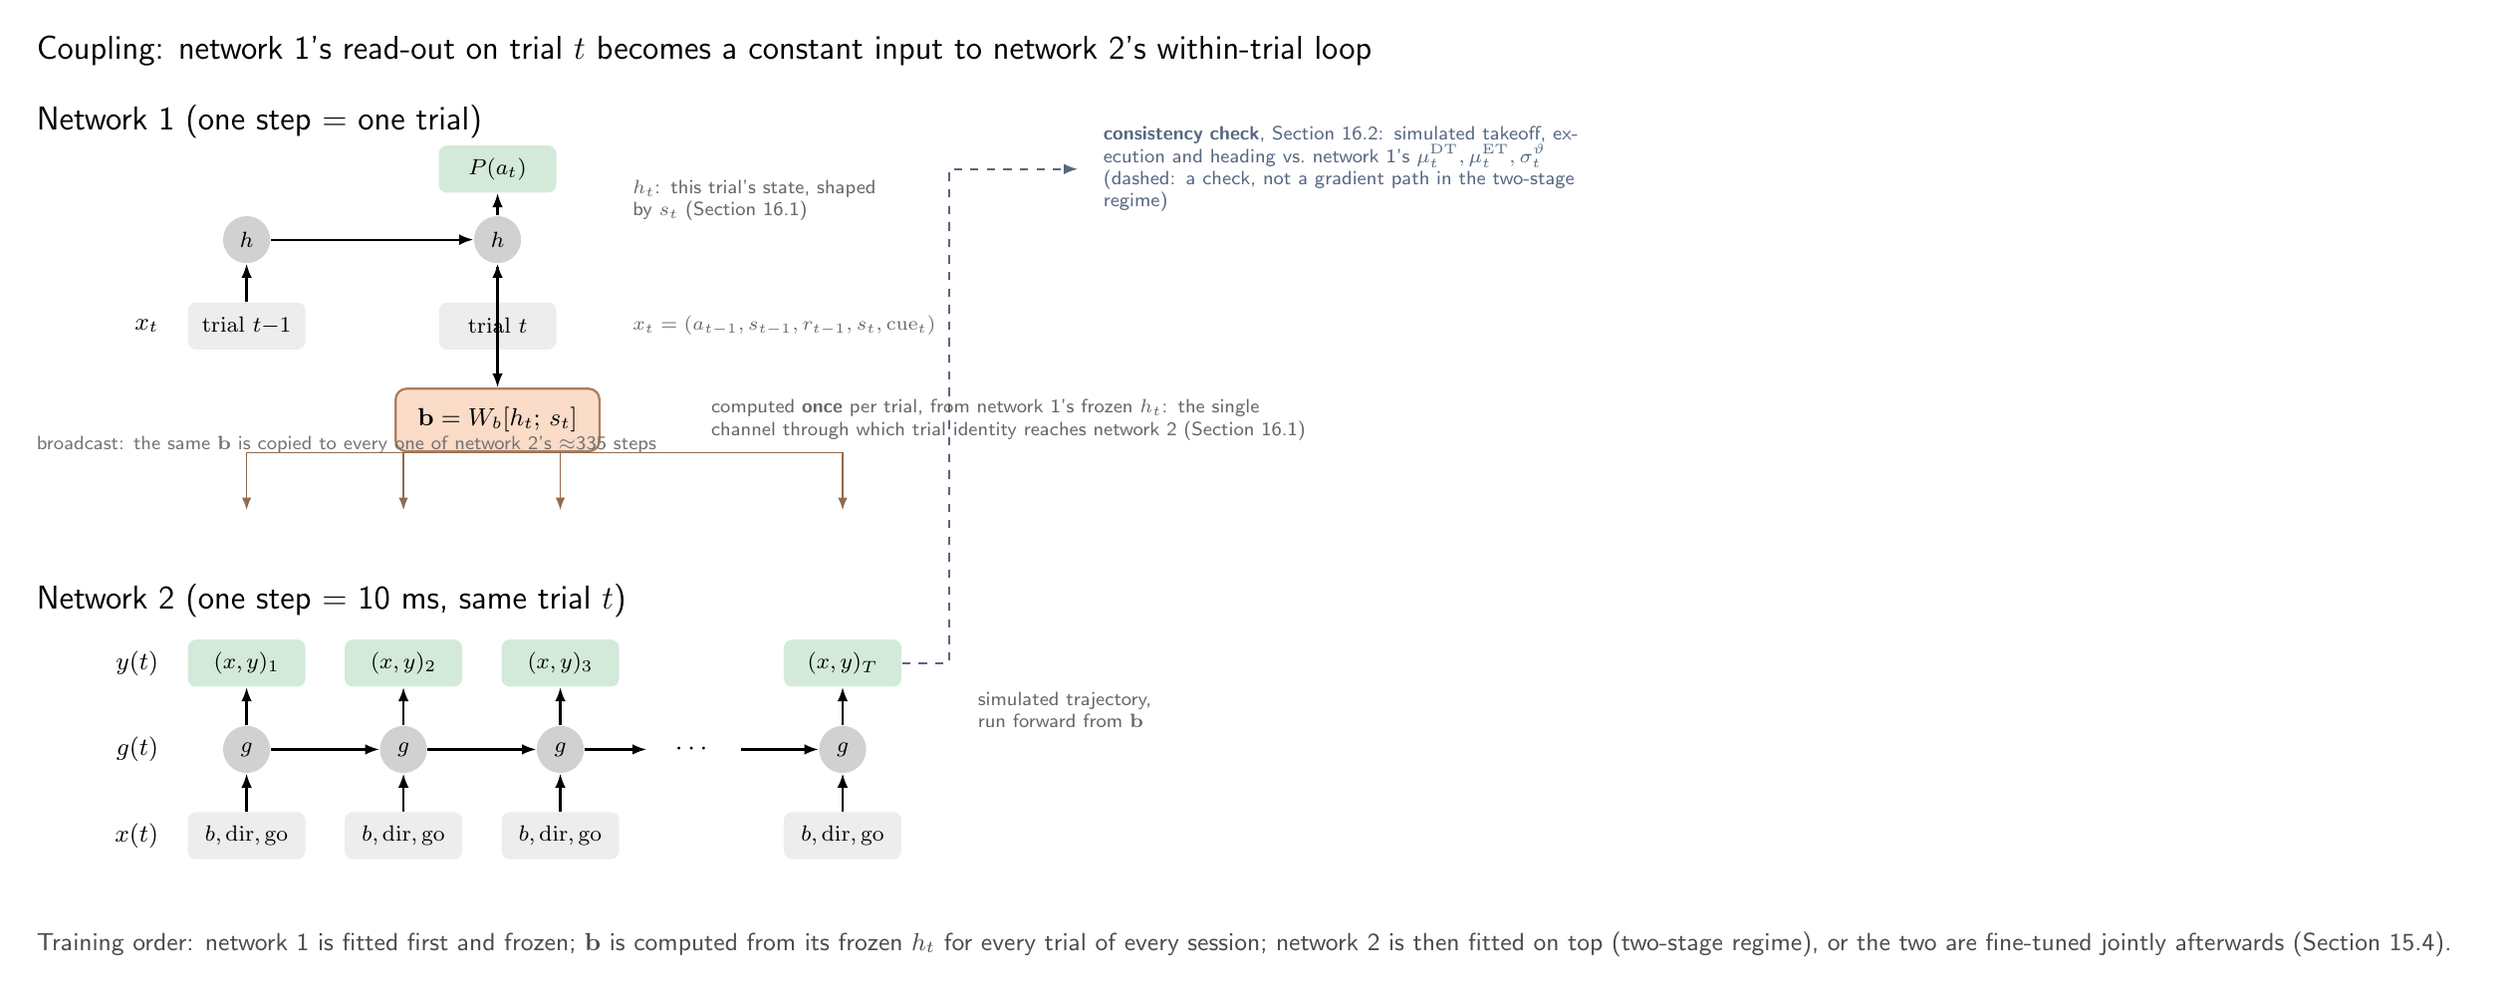
\begin{tikzpicture}[ctpanel,
  xin/.style={rounded corners=3pt, fill=black!7, draw=none, minimum width=1.5cm, minimum height=0.6cm, font=\footnotesize},
  hid/.style={circle, fill=black!18, draw=none, minimum size=0.6cm, inner sep=0pt, font=\footnotesize},
  bbox/.style={rounded corners=4pt, fill=catShort!45, draw=catShort!70!black, line width=0.8pt, minimum width=2.6cm, minimum height=0.8cm, font=\small},
  yout/.style={rounded corners=3pt, fill=catMid!45, draw=none, minimum width=1.5cm, minimum height=0.6cm, font=\footnotesize},
  rec/.style={-{Latex[length=1.8mm]}, line width=0.8pt},
  bc/.style={-{Latex[length=1.6mm]}, line width=0.6pt, catShort!60!black},
  chk/.style={-{Latex[length=1.8mm]}, line width=0.8pt, dashed, catLong!55!black},
  lab/.style={font=\sffamily\small, anchor=east},
  note/.style={font=\sffamily\scriptsize, text=black!60, align=left, anchor=west},
  rowtitle/.style={font=\sffamily\large, anchor=west},
]

\node[font=\sffamily\large, anchor=west] at (-2.4,10.0)
  {Coupling: network 1's read-out on trial $t$ becomes a constant input to network 2's within-trial loop};

% =====================================================================
% Row 1: network 1, trial loop (zoomed on trial t)
% =====================================================================
\begin{scope}[yshift=6.5cm]
  \node[rowtitle] at (-2.4,2.6) {Network 1 (one step = one trial)};
  \node[lab] at (-0.6,0) {$x_t$};
  \node[xin] (xprev) at (0.4,0) {trial $t{-}1$};
  \node[hid] (hprev) at (0.4,1.1) {$h$};
  \node[xin] (xnow) at (3.6,0) {trial $t$};
  \node[hid] (hnow) at (3.6,1.1) {$h$};
  \draw[rec] (xprev) -- (hprev);
  \draw[rec] (xnow) -- (hnow);
  \draw[rec] (hprev) -- (hnow);
  \node[yout] (ynow) at (3.6,2.0) {$P(a_t)$};
  \draw[rec] (hnow) -- (ynow);
  \node[note, text width=6.6cm] at (5.2,1.6) {$h_t$: this trial's state, shaped\\ by $s_t$ (Section 16.1)};
  \node[note, text width=6.6cm] at (5.2,0) {$x_t = (a_{t-1}, s_{t-1}, r_{t-1}, s_t, \mathrm{cue}_t)$};
\end{scope}

% =====================================================================
% b construction (below h_t, above the broadcast fan-out)
% =====================================================================
\node[bbox] (bbox) at (3.6,5.3) {$\mathbf{b} = W_b[h_t;\, s_t]$};
\draw[rec] (3.6,6.5+1.1-0.35) -- (bbox.north);
\node[note, text width=7.6cm] at (6.2,5.3) {computed \textbf{once} per trial, from network 1's frozen $h_t$: the single channel through which trial identity reaches network 2 (Section 16.1)};

\node[font=\sffamily\scriptsize, text=black!55, anchor=south west] at (-2.4,4.75)
  {broadcast: the same $\mathbf{b}$ is copied to every one of network 2's $\approx$335 steps};
\foreach \x in {0.4, 2.4, 4.4, 8.0}{
  \draw[bc] (bbox.south) -| (\x,4.15);
}

% =====================================================================
% Row 2: network 2, within-trial loop
% =====================================================================
\begin{scope}[yshift=0cm]
  \node[rowtitle] at (-2.4,3.0) {Network 2 (one step = 10 ms, same trial $t$)};
  \node[lab] at (-0.6,0)   {$x(t)$};
  \node[lab] at (-0.6,1.1) {$g(t)$};
  \node[lab] at (-0.6,2.2) {$y(t)$};
  \node[xin] (ma) at (0.4,0) {$b,\mathrm{dir},\mathrm{go}$};
  \node[hid] (ga) at (0.4,1.1) {$g$};
  \node[yout] (pa) at (0.4,2.2) {$(x,y)_1$};
  \node[xin] (mb) at (2.4,0) {$b,\mathrm{dir},\mathrm{go}$};
  \node[hid] (gb) at (2.4,1.1) {$g$};
  \node[yout] (pb) at (2.4,2.2) {$(x,y)_2$};
  \node[xin] (mc) at (4.4,0) {$b,\mathrm{dir},\mathrm{go}$};
  \node[hid] (gc) at (4.4,1.1) {$g$};
  \node[yout] (pc) at (4.4,2.2) {$(x,y)_3$};
  \node at (6.1,1.1) {$\cdots$};
  \node[xin] (md) at (8.0,0) {$b,\mathrm{dir},\mathrm{go}$};
  \node[hid] (gd) at (8.0,1.1) {$g$};
  \node[yout] (pd) at (8.0,2.2) {$(x,y)_T$};
  \foreach \n in {a,b,c,d}{ \draw[rec] (m\n) -- (g\n); \draw[rec] (g\n) -- (p\n); }
  \draw[rec] (ga) -- (gb); \draw[rec] (gb) -- (gc);
  \draw[rec] (gc) -- (5.5,1.1); \draw[rec] (6.7,1.1) -- (gd);
  \node[note, text width=6.0cm] at (9.6,1.6) {simulated trajectory,\\ run forward from $\mathbf{b}$};
\end{scope}

% =====================================================================
% feedback check (dashed, not a gradient path in the two-stage regime)
% =====================================================================
\draw[chk] (pd.east) -- ++(0.6,0) |- (11.0,6.5+2.0);
\node[font=\sffamily\scriptsize, text=catLong!55!black, anchor=west, align=left, text width=6.4cm] at (11.2,6.5+2.0)
  {\textbf{consistency check}, Section 16.2: simulated takeoff, execution and heading vs.\ network 1's $\mu^{\mathrm{DT}}_t, \mu^{\mathrm{ET}}_t, \sigma^{\vartheta}_t$ (dashed: a check, not a gradient path in the two-stage regime)};

\node[align=left, anchor=north west, font=\sffamily\small, text=black!70] at (-2.4,-1.1) {%
  Training order: network 1 is fitted first and frozen; $\mathbf{b}$ is computed from its frozen $h_t$ for every trial of every
  session; network 2 is then fitted on top (two-stage regime), or the two are fine-tuned jointly afterwards (Section 15.4).
};

\end{tikzpicture}
\end{document}
